\begin{frame}{2004 CPU}
    \begin{tikzpicture}[scale=1.25]
\clip (1,0) rectangle (14, 7);
\node[anchor=south west] (diePhoto) at (0,0) {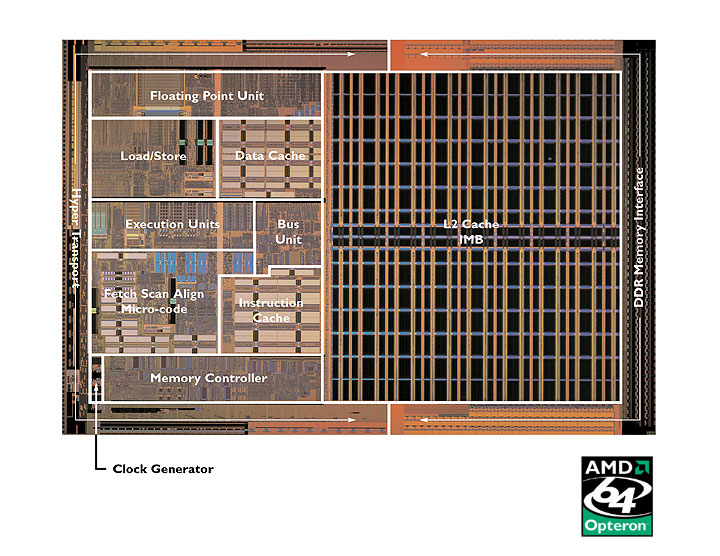
\includegraphics[width=11.25cm]{Opteron_die_labelled.jpg}};
%\draw[red] (0, 0) grid (9,7);
    \newcommand{\pyrShift}{0.5cm}
\onslide<2->{
    \draw[fill=red,opacity=0.6] (1.9,6.2) rectangle (2.4,5.8);
    \draw[fill=red,opacity=0.6] (1.7,4.2) rectangle (1.9,4.6);

    \begin{scope}[xshift=\pyrShift]
    \draw[fill=red!60!white] (10,7) -- (9.75,6.5) -- (10.25,6.5) -- cycle;
    \node[anchor=west] at (10.1, 6.75) {Registers};
    \end{scope}
}
\onslide<3->{
    %\draw[fill=orange,opacity=0.6] (2.95,2.7) rectangle (4.2,3.6);
    \draw[fill=orange,opacity=0.6] (2.95,2.7) -| (4.2,3.8) -| (3.6,3.65) -- (2.95,3.65) -- (2.95,2.7);
    \draw[fill=orange,opacity=0.6] (2.95,4.6) rectangle (4.2,5.6);

    \begin{scope}[xshift=\pyrShift]
    \draw[fill=orange!60!white] (9.5,6) -- (9.75,6.5) -- (10.25,6.5) -- (10.5,6) -- cycle;
    \node[anchor=west] at (10.35,6.25) {L1 cache};
    \end{scope}
}
\onslide<4->{
    \draw[fill=yellow,opacity=0.6] (4.2,2.1) rectangle (7.9,6.25);
    
    \begin{scope}[xshift=\pyrShift]
    \draw[fill=yellow!60!white] (9.25,5.5) -- (9.5,6) -- (10.5,6) -- (10.75,5.5) -- cycle;
    \node[anchor=west] at (10.6,5.75) {L2 cache};
    \end{scope}
}
\onslide<6->{
    \begin{scope}[xshift=\pyrShift]
    \draw[pattern color=green!60!white,pattern=north west lines] (9.0,5.) -- (9.25,5.5) -- (10.75,5.5) -- (11.,5.) -- cycle;
    \node[anchor=west] at (10.85,5.25) {L3 cache};
    \draw[fill=blue!60!white] (8.5,4.) -- (9.,5.) -- (11,5.) -- (11.5,4.) -- cycle;
    \node[anchor=center,align=center] at (10.,4.5) {main\\memory};
    \end{scope}
}
\onslide<7->{
    \begin{scope}[xshift=\pyrShift]
    \fill[white,opacity=0.9] (7.0,4.5) rectangle (8.4,10.0);
    \begin{scope}[font=\fontsize{10}{11}\selectfont]
        \node[anchor=east] at (9.,6.75) {$<1$ ns};
        \node[anchor=east] at (9.,6.25) {$\sim1$ ns};
        \node[anchor=east] at (9.,5.75) {$\sim5$ ns};
        \node[anchor=east] at (9.,5.25) {$\sim20$ ns};
        \node[anchor=east] at (9.,4.75) {$\sim100$ ns};
    \end{scope}
    \end{scope}
}
\end{tikzpicture}
    \imagecredit{Image: approx 2004 AMD press image of Opteron die; \\ approx register location via chip-architect.org (Hans de Vries)}
\end{frame}

% FIXME: colors consistent with previous slide
\begin{frame}{memory hierarchy overview}
\begin{tikzpicture}
    \begin{scope}[xscale=0.8,yscale=1.2]
        \draw[ultra thick] (-1,-1) -- (-7, -7) -- (7, -7) -- (1,-1) -- cycle;
        \foreach \x/\lbl in {
                2/registers,
                3/{level 1 (L1) cache},
                4/{level 2 (L2) cache},
                5/{level 3 (L3) cache},
                6/main memory,
                7/hard disk or SSD
            } {
            \draw[thick] (-\x, -\x) -- (\x, -\x);
            \node[anchor=south] at (0, -\x) {\lbl};
        }
        \tikzset{
            >=Latex
        }
        \draw[->,thick] (3, -2) -- (6, -5) node[below right] {bigger and slower};
        \node[anchor=west] at (3, -2) {faster and smaller};
    \end{scope}
\end{tikzpicture}
\end{frame}

\begin{frame}{memory hierarchy goal}
    \begin{itemize}
    \item size of largest, slowest storage
    \item speed of smallest, fastest storage
        \vspace{.5cm}
    \item not actually possible, but can get pretty close due to locality
    \end{itemize}
\end{frame}

\begin{frame}{memory hierarchy numbers}
from a system like my desktop: \\
    {\small (note: multiple parallel accesses and/or sequential accesses needed to achieve maximum bandwidths)} \\
\begin{tabular}{l|lll}
level & time/access & maximum read bandwidth \\ \hline
registers & 0.3 ns & $\sim$ 645 GB/s (per core)\\
L1 cache & 1.2 ns & $\sim$ 199 GB/s (per core) \\
L2 cache & 3.6 ns & $\sim$ 110 GB/s (per core)\\
L3 cache & $\sim$ 13 ns & $\sim$ 54 GB/s \\
main memory & $\sim$ 64 ns & $\sim$ 25 GB/s \\
hard disk & $\sim$ 5$\;$000$\;$000 ns & $\sim$ 0.1 GB/s \\
\end{tabular}
\end{frame}

